\section[Problem 1]{Problem 1: Area-Oriented Recognition of Newly Inundated Area}
\label{sec:q1}

\subsection{Independent Samples by Spatially Blocked Cross-Validation}

The problem asks for evaluation ``using independent samples''. Neighbouring tiles share the same flood and the same fields, so a random split of tiles, let alone of pixels, would put near-copies of a test tile into training. The 1000 tiles lie on a regular grid of $199\times42$ tile positions. We group them into 67 blocks of $5\times5$ positions (Assumption~1) and assign the blocks to five folds by a greedy stratified rule that balances tile count and flood area. For outer fold $k=0,\dots,4$,
\begin{equation}
\begin{split}
\mathcal T^{test}_k&=\mathcal F_k,\\
\mathcal T^{cal}_k&=\mathcal F_{(k+1)\bmod 5},\\
\mathcal T^{train}_k&=\Big\{t\notin\mathcal F_k\cup\mathcal F_{k+1}:\ \min_{s\in\mathcal F_k\cup\mathcal F_{k+1}}\lVert g_t-g_s\rVert_\infty>1\Big\},
\end{split}
\label{eq:folds}
\end{equation}
where $\mathcal F_k$ is the set of tiles in fold $k$ and $g_t$ the grid position of tile $t$. The calibration fold is used for every choice that would otherwise peek at the test data (threshold, early stopping, isotonic map, conformal quantile), and the Chebyshev buffer of one tile removes the training tiles that touch a test or calibration tile. The resulting test folds hold 194, 200, 202, 202 and 202 tiles with flood shares 0.184--0.202, and 170--196 buffer tiles are dropped from each training set. Every tile is tested exactly once, so all metrics below are pooled over the 1000 held-out tiles. This design follows the recommendation of blocked cross-validation for spatially structured data~\cite{roberts2017crossvalidation}.

\subsection{Two Recognizers of Different Kinds}

\textbf{Baseline A: physics two-stage rule.} The classical route estimates post-flood water from SAR and subtracts pre-flood water from optics. Each tile is cut into 16 sub-blocks of $64\times64$ pixels, and Otsu's threshold $\tau_b$ on $\tilde z$ is accepted for a sub-block only if its two classes are clearly bimodal~\cite{martinis2009splitbased},
\begin{equation}
D_b=\frac{\sqrt2\,|\mu_1-\mu_2|}{\sqrt{s_1^2+s_2^2}}>2\quad\text{and}\quad \min(n_1,n_2)\ge0.1\,(n_1+n_2),
\label{eq:ashman}
\end{equation}
where $\mu_i,s_i,n_i$ are the class means, standard deviations and sizes (Ashman's $D$). The tile threshold is the median of the accepted $\tau_b$, with a fold-level median as fallback. Then $\hat F_A=\{\tilde z<\tau\}\setminus\{\mathrm{NDWI}>0\}$, and components smaller than 10 pixels are removed. Labels are not used at all, so baseline A measures how far a rule without training gets.

\textbf{Baseline B: LightGBM pixel classifier.} The second recognizer learns $\Pr(y_p=1\mid\boldsymbol x_p)$ from the 19 features of Section~\ref{sec:data_def} with gradient-boosted trees~\cite{lightgbm2020package}. Because labels mark new inundation, the classifier learns $F$ directly. Up to 2000 pixels per training tile are drawn, half positive and half negative where possible (about 0.8\,M rows per fold), which handles the imbalance; the prior shift this causes is absorbed by the threshold
\begin{equation}
\tau_k=\arg\max_{\tau\in\{0.05,0.06,\dots,0.95\}}\ \mathrm{F1}\big(\mathcal T^{cal}_k;\tau\big),
\label{eq:tau_f1}
\end{equation}
chosen on the calibration fold. The trees use 63 leaves, learning rate 0.05 and early stopping after 50 rounds on calibration pixels; the selected thresholds were 0.46, 0.58, 0.77, 0.40 and 0.59 with 390--1211 trees.

\subsection{Pixel and Area Metrics}

Pixel metrics (overall accuracy OA, precision, recall, F1, IoU and Cohen's $\kappa$) come from the pooled confusion matrix. The area metrics follow the problem's emphasis and use the tile error $e_t=\hat A_t-A_t$ with $A_t=\sum_{p\in t}a_py_p$:
\begin{equation}
\begin{split}
\Delta A&=\sum_te_t,\qquad
\mathrm{RAE}=\frac{\sum_t\hat A_t-\sum_tA_t}{\sum_tA_t},\\
\mathrm{MAE}_A&=\frac1T\sum_t|e_t|,\qquad
\mathrm{RAE}_t=\frac{e_t}{A_t}\ \ (A_t\ge0.05\ \mathrm{km}^2).
\end{split}
\label{eq:area_metrics}
\end{equation}
RAE measures bias of the total, while MAE$_A$ measures how wrong a single tile is; the two differ because tile errors of opposite sign cancel in $\Delta A$ (identity \eqref{eq:fpfn_identity}). The floor of 0.05\,km$^2$ (about 1\% of a tile) avoids dividing by near-zero reference areas. Agreement is also shown by the Bland--Altman bias $\bar e$ and limits $\bar e\pm1.96s_e$~\cite{bland1986agreement}.

\subsection{Recognition Results on 1000 Held-out Tiles}

Table~\ref{tab:q1_metrics} gives the pooled results. The two baselines differ by a factor of more than two in IoU and by a factor of 15 in total area bias.

\begin{table}[H]
\centering
\caption{Held-out performance of the Problem 1 recognizers}
\label{tab:q1_metrics}
\resizebox{\textwidth}{!}{%
\begin{tabular}{lccccccccc}
\toprule
Model & OA & Precision & Recall & F1 & IoU & $\kappa$ & RAE & MAE$_A$ (km$^2$) & median $|\mathrm{RAE}_t|$ \\
\midrule
A: split-Otsu $-$ NDWI & 0.634 & 0.308 & 0.740 & 0.435 & 0.278 & 0.227 & $+1.406$ & 1.756 & 2.84 \\
B: LightGBM (M0) & 0.900 & 0.717 & 0.783 & 0.749 & 0.598 & 0.686 & $+0.092$ & 0.430 & 0.52 \\
\bottomrule
\end{tabular}}
\end{table}

The 1000 reference tiles contain 933.41\,km$^2$ of new inundation. LightGBM returns 1019.12\,km$^2$, 9.2\% above the reference (an excess of 85.71\,km$^2$). Its fold-level RAE ranges from $-13.9\%$ to $+34.6\%$ (IoU 0.546--0.622), so the pooled value hides a spread that a single random split would never show. Baseline A finds 74\% of the flooded pixels but also labels 2245.66\,km$^2$ as new water, 2.4 times the reference. The reason is visible in its own diagnostic: the Ashman test of \eqref{eq:ashman} passes on 92\% of the sub-blocks, also on tiles without water, because dark fields and bright villages form a bimodal histogram too. We report this as a finding about the baseline and did not tune it on the test labels.

The pooled numbers do not tell where on a tile the errors occur. Fig.~\ref{fig:q1_visual_cmp} therefore shows four held-out tiles of increasing flood share, each predicted by the model of the fold in which it was a test tile; columns 4--6 are confusion maps (true positives, FP, FN) of baseline A, LightGBM and the final Problem~2 model M6.

\begin{figure}[H]
  \centering
  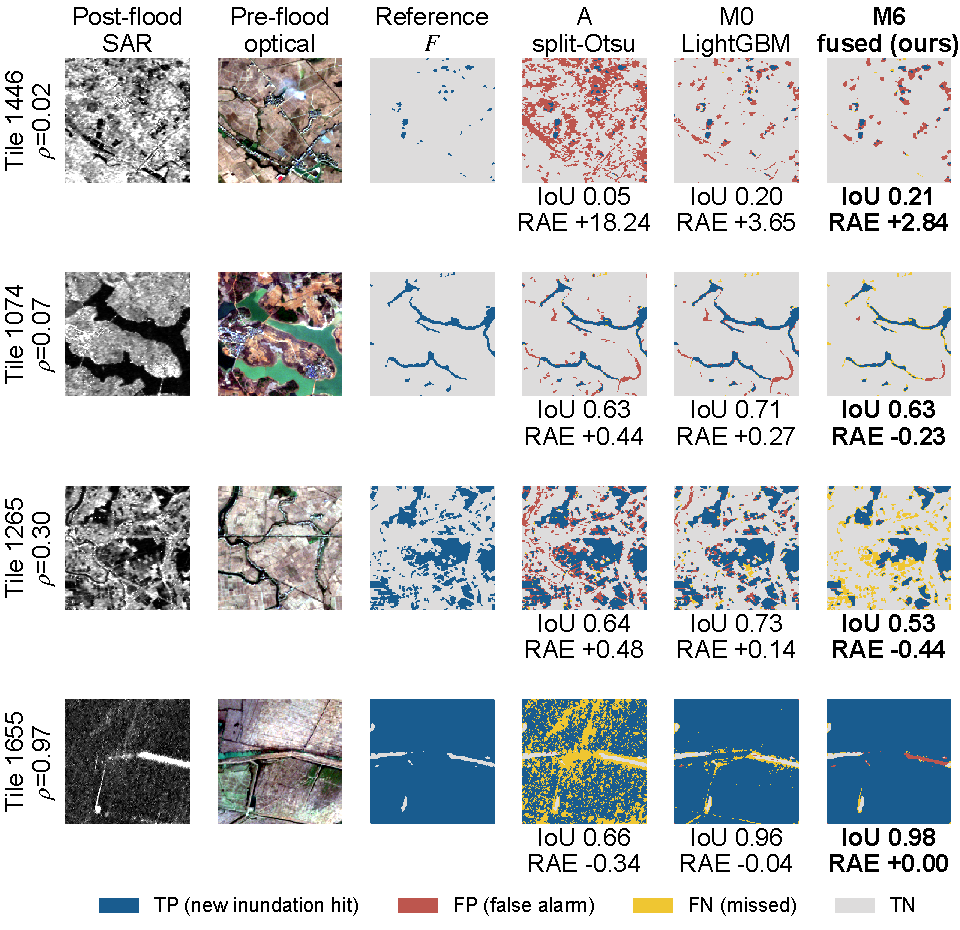
\includegraphics[width=0.98\textwidth,keepaspectratio]{../figures/fig_q1_visual_cmp.pdf}
  \caption{Held-out predictions on four official tiles}
  \label{fig:q1_visual_cmp}
\end{figure}

On tile 1446, where only 1.8\% of the area is flooded, every method fails in the same way: baseline A reaches IoU 0.052 with a relative area error of $+18.2$, and LightGBM still predicts 4.65 times the reference area (RAE$_t=+3.65$), because a few dark fields form most of the prediction. On the medium tiles 1074 ($\rho=7.4\%$) and 1265 ($\rho=30.5\%$) LightGBM has IoU 0.707 and 0.734 and area errors of $+27\%$ and $+15\%$; the false alarms sit along field edges and the misses inside vegetated patches. On the almost fully flooded tile 1655 ($\rho=97.3\%$) LightGBM reaches IoU 0.959 and M6 0.980 with an area error of $+0.4\%$. Relative area error is therefore driven by small reference areas, not by poor pixel classification, which is why the per-tile error has to be read together with the total.

Every held-out tile is also exported as a mask, and Fig.~\ref{fig:q1_pred_set} shows five of them that do not appear in Fig.~\ref{fig:q1_visual_cmp}, spanning a reference share from 2\% to 94\%. At the almost dry tile 1720 baseline A labels half of the tile as water, while LightGBM stays at 5.2\%; at the flooded tiles both follow the water outline.

\begin{figure}[H]
  \centering
  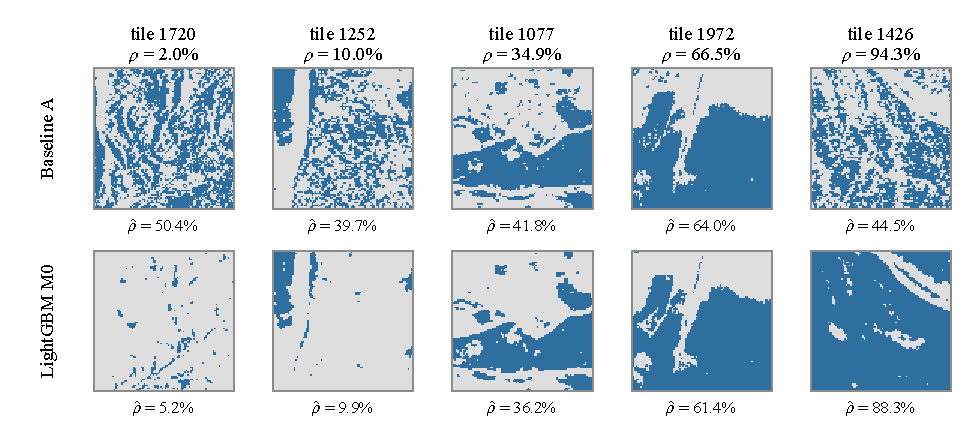
\includegraphics[width=0.95\textwidth,keepaspectratio]{../figures/fig_q1_pred_examples.pdf}
  \caption{Exported tile masks: baseline A (top) and LightGBM M0 (bottom), new water in blue}
  \label{fig:q1_pred_set}
\end{figure}

That observation becomes quantitative in the Bland--Altman plot of Fig.~\ref{fig:q1_area_agreement}, which compares estimated and reference tile areas for all 1000 tiles.

\begin{figure}[H]
  \centering
  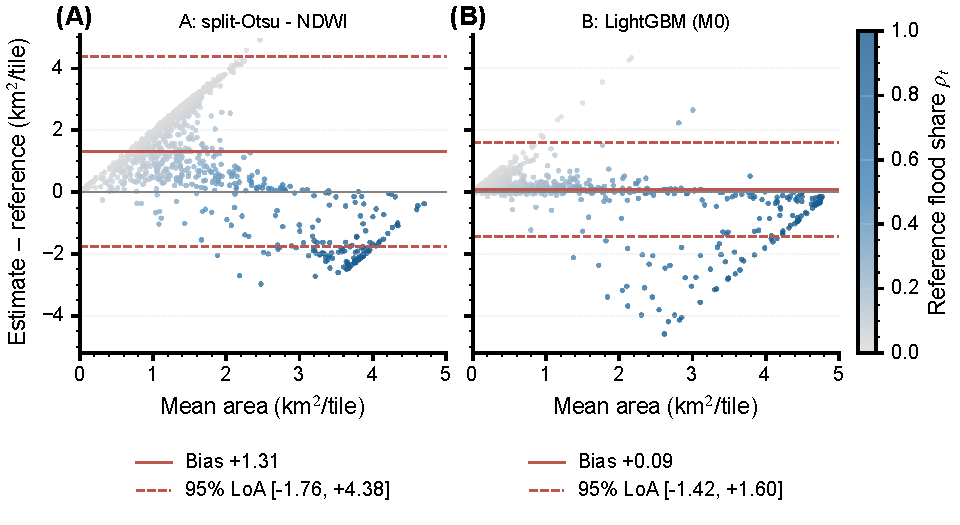
\includegraphics[width=0.95\textwidth,keepaspectratio]{../figures/fig_q1_area_agreement.pdf}
  \caption{Bland--Altman agreement of tile new-inundation area}
  \label{fig:q1_area_agreement}
\end{figure}

Baseline A over-estimates by $+1.31$\,km$^2$ per tile on average, with 95\% limits of $-1.76$ to $+4.38$\,km$^2$, and the excess grows on tiles with little reference flood (panel a). LightGBM removes most of the bias ($+0.086$\,km$^2$) but its limits of agreement, $-1.42$ to $+1.60$\,km$^2$, are still wide compared with the mean tile area of 4.91\,km$^2$. The scatter is widest on tiles with intermediate flood share, where fragmented flood patches meet dark fields. A model whose area error has to be small on each assessment unit, not only in the city total, therefore needs spatial context, which motivates the convolutional model of Problem~2.

\subsection{False Positives and False Negatives by Land Cover}

The problem asks how FP and FN under different land covers affect the area. With land-cover stratum $c$, identity \eqref{eq:fpfn_identity} decomposes exactly:
\begin{equation}
\mathrm{FP}_c=\sum_{p\in c}a_p\hat y_p(1-y_p),\qquad
\mathrm{FN}_c=\sum_{p\in c}a_p(1-\hat y_p)y_p,\qquad
\Delta A=\sum_c(\mathrm{FP}_c-\mathrm{FN}_c).
\label{eq:fpfn_strata}
\end{equation}
The attachment carries no land cover, so the strata come from ESA WorldCover 2021, read for each tile footprint and resampled by nearest neighbour; this describes the pre-flood land state under the assumption that it did not change much between 2021 and the image date. Table~\ref{tab:q1_fpfn} lists the decomposition for LightGBM.

\begin{table}[H]
\centering
\caption{Area decomposition of LightGBM errors by pre-flood land cover (km$^2$)}
\label{tab:q1_fpfn}
\begin{tabular}{lcccc}
\toprule
Stratum & Reference $F$ & FP & FN & Net FP$-$FN \\
\midrule
Tree & 33.46 & 79.80 & 4.93 & $+74.87$ \\
Shrub / grassland & 53.92 & 23.43 & 7.65 & $+15.77$ \\
Cropland & 379.62 & 105.59 & 59.09 & $+46.50$ \\
Built-up & 8.79 & 19.38 & 1.81 & $+17.57$ \\
Bare & 7.97 & 7.70 & 1.15 & $+6.54$ \\
Permanent water & 156.06 & 26.80 & 50.91 & $-24.11$ \\
Wetland & 293.59 & 25.46 & 76.89 & $-51.43$ \\
\bottomrule
\end{tabular}
\end{table}

The table shows two opposite mechanisms. On dry land covers the model raises false alarms: tree cover contributes 79.80\,km$^2$ of FP against only 33.46\,km$^2$ of real new flood, built-up land 19.38\,km$^2$ against 8.79\,km$^2$. Radar shadow behind tree canopies and smooth surfaces in villages look as dark as water. On wet land covers it misses flood: in wetland and areas that WorldCover maps as permanent water, the net error is $-51.43$ and $-24.11$\,km$^2$, because water that rose over a wetland or a lake margin is hard to tell from the water that was already there. The positive and negative nets cancel to the total $+85.71$\,km$^2$; the worst strata by absolute net error are tree, wetland and cropland.

\subsection{Key Factors of Area Accuracy}

To find the factors behind the tile error, each held-out tile gets label-free descriptors (raw SAR mean and standard deviation, share of bimodal sub-blocks, ENL, mean NDVI, WorldCover shares, optical invalid share) together with the reference flood share and the boundary density of the reference flood (perimeter over area). A gradient-boosted regressor on the same spatial folds predicts $|e_t|$ from these descriptors (out-of-fold $R^2=0.417$), and TreeSHAP values~\cite{lundberg2020trees} rank the factors. Fig.~\ref{fig:q1_error_drivers} combines this ranking with the land-cover decomposition.

\begin{figure}[H]
  \centering
  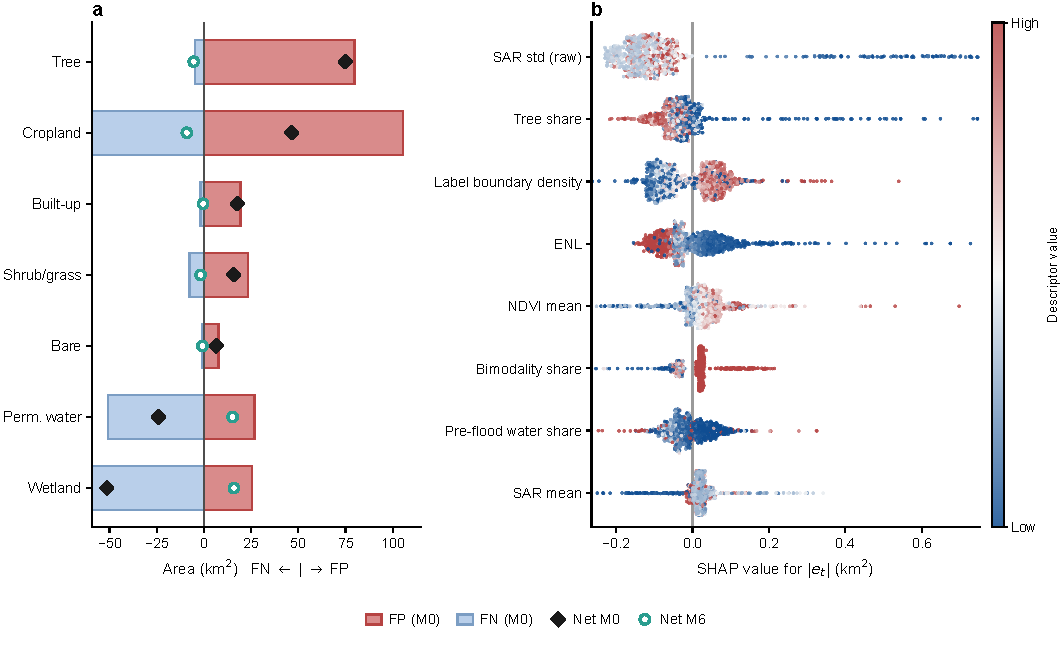
\includegraphics[width=0.98\textwidth,keepaspectratio]{../figures/fig_q1_error_drivers.pdf}
  \caption{Error structure of the Problem 1 model}
  \label{fig:q1_error_drivers}
\end{figure}

Panel (a) of Fig.~\ref{fig:q1_error_drivers} repeats the FP/FN bars of Table~\ref{tab:q1_fpfn} and adds the net error of the Problem~2 model M6 for later comparison. Panel (b) ranks the drivers of absolute tile error by mean $|\mathrm{SHAP}|$: the raw SAR standard deviation is first (0.196), followed by tree share (0.077), boundary density of the flood (0.074), ENL (0.073), NDVI mean (0.057), bimodality share (0.050) and pre-flood water share (0.045). High SAR variance and low ENL mean strong speckle and mixed scattering, tree share is the FP mechanism of Table~\ref{tab:q1_fpfn}, and a high boundary density means fragmented flood that a pixel classifier cuts into pieces. For the signed error the reference flood share comes first, i.e. the model over-estimates on lightly flooded tiles and under-estimates on heavily flooded ones.

A harder notion of independence holds out a whole spatial cluster. Training on three of the four clusters and testing on the fourth lowers the pooled IoU from 0.598 to 0.508 and F1 from 0.749 to 0.674, and the cluster RAE is $+26\%$ on the 512-tile cluster and $+15\%$ on the 450-tile cluster. Transfer to an unseen region thus costs about 0.09 IoU and adds a positive area bias, which is what Problem~3 has to face in Guangxi.

These analyses define what Problem~2 must fix. The 397 tiles with $A_t\ge0.05$\,km$^2$ and $|\mathrm{RAE}_t|>0.5$ under LightGBM form the ``hard set''. The dominant error mechanisms are dark dry surfaces (tree, built-up) and fragmented or vegetated flood, both of which need spatial context and the optical land state, and the dominant error measure is a positive total bias that pixel-wise training does not control.
